%================================================================
\documentclass[symmetry,article,submit,moreauthors,pdftex]{Definitions/mdpi} 

%=================================================================
% MDPI internal commands
\firstpage{1} 
\makeatletter 
\setcounter{page}{\@firstpage} 
\makeatother
\pubvolume{1}
\issuenum{1}
\articlenumber{0}
%\doinum{}
\pubyear{2021}
\copyrightyear{2020}
%\externaleditor{Academic Editor: Firstname Lastname} % For journal Automation, please change Academic Editor to "Communicated by"
\datereceived{} 
\dateaccepted{} 
\datepublished{} 
%\datecorrected{} % Corrected papers include a "Corrected: XXX" date in the original paper.
%\dateretracted{} % Corrected papers include a "Retracted: XXX" date in the original paper.
\hreflink{https://doi.org/} % If needed use \linebreak
%=================================================================
%% Please use the following mathematics environments: Theorem, Lemma, Corollary, Proposition, Characterization, Property, Problem, Example, ExamplesandDefinitions, Hypothesis, Remark, Definition, Notation, Assumption
%% For proofs, please use the proof environment (the amsthm package is loaded by the MDPI class).
\usepackage{listings}
\usepackage{subfigure}
%=================================================================
% Full title of the paper (Capitalized)
\Title{Optimal Fuzzy Controller Design for Autonomous Robot Path Tracking using Population-based Metaheuristics}

% MDPI internal command: Title for citation in the left column
\TitleCitation{Optimal Fuzzy Controller Design for Autonomous Robot Path Tracking using Genetic Algorithms}

% Author Orchid ID: enter ID or remove command
\newcommand{\orcidauthorA}{0000-0003-0430-8152} % Add \orcidA{} behind the author's name
\newcommand{\orcidauthorB}{0000-0002-2593-1114} % Add \orcidB{} behind the author's name
\newcommand{\orcidauthorC}{0000-0002-7385-5689} % Add \orcidB{} behind the author's name
\newcommand{\orcidauthorD}{0000-0002-1385-9741} % Add \orcidB{} behind the author's name

% Authors, for the paper (add full first names)
\Author{Alejandra Mancilla $^{1}$\orcidA{},
  Mario Garc\'{i}a-Valdez $^{1,}$*\orcidB{},
  Oscar Castillo$^{1}$\orcidC{} 
  and JJ Merelo-Guerv\'{o}s$^{2}$\orcidD{}}

% MDPI internal command: Authors, for metadata in PDF
\AuthorNames{Alejandra Mancilla, Mario Garc\'{i}a-Valdez, Oscar Castillo and JJ Merelo-Guerv\'{o}s}

% MDPI internal command: Authors, for citation in the left column
\AuthorCitation{Mancilla, A.; Garc\'{i}a-Valdez, M.; Castillo, O.; Merelo-Guerv\'{o}s, J.J.}
% If this is a Chicago style journal: Lastname, Firstname, Firstname Lastname, and Firstname Lastname.

% Affiliations / Addresses (Add [1] after \address if there is only one affiliation.)
\address{%
$^{1}$ \quad Tijuana Institute of Technology;\{alejanda.mancilla,mario,ocastillo\}@tectijuana.edu.mx\\
$^{2}$ \quad University of Granada; jmerelo@ugr.es}

% Contact information of the corresponding author
\corres{Correspondence: mario@tectijuana.edu.mx; Tel.:+52-664-123-7806 (M.G.V.)}

% Current address and/or shared authorship
%\simplesumm{} % Simple summary

\conference{INFUS-21} % An extended version of a conference paper

% Abstract (Do not insert blank lines, i.e. \\)

\abstract{ In this work we propose, through the use of population-based
metaheuristics, an optimization method that solves the problem of autonomous path
tracking using a rear-wheel fuzzy logic controller. This approach enables the
design of controllers using rules that are linguistically familiar to human
users. Moreover, a new technique that uses three different paths to validate the
performance of each candidate configuration is presented. We extend on our
previous work by adding two more membership functions to the previous fuzzy
model, intending to have a finer-grained adjustment. We tuned the controller 
using several well-known metaheuristic methods, Genetic Algorithms (GA),
Particle Swarm Optimization (PSO), Grey Wolf Optimizer (GWO), Harmony Search (HS), and the recent 
Aquila Optimizer (AO) and Arithmetic Optimization Algorithms. Experiments show that,
compared to a published control law, % control law? - JJ
the proposed fuzzy controllers have better RMSE-measured performance. Nevertheless, the
experiments also highlight problems with the common practice of evaluating the
performance of fuzzy controllers with a single problem case and performance
metric, resulting in controllers that tend to be overtrained.}

% Keywords
\keyword{Fuzzy Systems; Fuzzy Control; Bioinspired Algorithms.}

\begin{document}

\section{Introduction}

Proposed by Lofti Zadeh \cite{goguen_zadeh_1973}, fuzzy logic introduces the
concepts of fuzzy sets and fuzzy logic operators \cite{zadeh1996fuzzy}.
Contrary to boolean logic, in which an element is a member of a set or is not,
in fuzzy logic, elements have a degree of membership to many sets. Fuzzy logic uses
so-called membership functions (MFs) to assign a numerical value to each set
member, indicating their degree of membership. MFs must be defined for each
linguistic variable; these variables can be used in a rule-based system to
express knowledge in a way similar to natural language, for instance, the rule
``if distance is near'' uses the linguistic variable distance, with a fuzzy MF
assigning a degree of membership to the set near to each element of the
distance domain; for instance, for 2mm and 50mm the function will assign the
following degrees of membership: near(2)=.92 and near(50)=.40. These rule based
systems can express complex relationships well suited for control applications.

That is why, since the earlier years of fuzzy logic theory, fuzzy inference
systems \cite{driankov_introduction_2013} have been applied to control problems
\cite{mamdani1974application,king1977application,passino1998fuzzy,driankov_introduction_2013},
in many research projects \cite{yang_improved_2003,driankov_fuzzy_2013} and
commercial systems.

Many papers address the problem of path tracking control with fuzzy logic, the
earlier works used simple fuzzy rules to make adjustments to linear controllers
\cite{lee_practical_2003}, or integrated fuzzy logic to a complex adaptive
controller \cite{sanchez1997adaptive}. Meng \cite{bi_control_2020} proposes a
Fuzzy PID (proportional–integral–derivative) Controller algorithm to a
two-degree-of-freedom arm robot. Antonelli et al.
\cite{antonelli_fuzzy-logic-based_2007} propose a set of rules to emulate the
way humans drive, using as inputs of curve and distance to the system.  We have
also reviewed works where authors use controllers for the follow-up and planning
of routes. For example, using a simplified kinematic model of the bicycle type
using the control law for the navigation and follow-up of a path
\cite{laumond_robot_1998}, in work presented by Beleño et al.
\cite{beleno_planeacion_2014} they propose the planning and tracking of the
trajectories of a land vehicle based on the steering control in a natural
environment.  Guerrero-Castellanos et al.
\cite{guerrero-castellanos_trajectory_2014} addresses the path following problem
for the robot (3, 0) based on its kinematic model and proposes a solution by
designing a control strategy that mainly considers the maximum permitted levels
of the control signal.

An essential caveat of applying fuzzy control strategies to real-world problems
is that we require the use of optimization or adaptive techniques to tune some
aspects of the fuzzy inference system.  From the membership functions (MFs)
that define the linguistic variables, to the definition of a rule-based
system, including a defuzzification method
\cite{xia2019command,isaka1988design}. 

Tuning is needed because the fuzzy controllers' performance is highly dependent
on the parameters of the fuzzy system used. Moreover, the option of making a
manual selection of these parameters is difficult because the search space is
of considerable size and requires the validation of establishing the
controller's performance by running time-consuming simulations.  Evolutionary
Algorithms (EAs) and other population-based metaheuristics are often employed in tuning 
Fuzzy Inference Systems (FIS) % Define this. Is it Fuzzy inference systems? - JJ
\cite{martinez-soto_bio-inspired_2012,DBLP:conf/evoW/SalemMGG18}.

Population-based metaheuristics, are stochastic techniques that search for
optimal solutions by using two strategies: exploration and exploitation.
Exploration searches the space globally, avoiding to be trapped in a local
optima, while exploitation, searches locally for nearby promising solutions.
Genetic Algorithms (GAs) are the canonical representatives of population-based
metaheuristics \cite{holland1992genetic}.  GAs work on a set of potential
solutions called a population that is evolved for a certain number of
generations until a suitable or optimal solution is found
\cite{muelas_algoritmos_2009}.  In each generation, potential solutions
(individuals) are evaluated, and then surviving individuals reproduce through
genetic crossover (exploration) and mutation operators (exploitation) to
generate new offspring.  Finally, there is a replacement mechanism to select
the most adapted offspring and used them to generate a new generation of the
population.  Most population-based metaheuristics, create an initial set of
random candidate solutions, then these are evaluated against a quality
function, then taking the quality and the position or structure of each
solution, a nature-inspired metaheuristic is applied to generate a new set of
candidates. 

Population-based metaheuristics have been extensively used for structural
optimization tasks \cite{perez2007particle,durgun2012structural,yildiz2012new,geem2005harmony}, 
together with more traditional gradient-based algorithms. These nature-inspired  
metaheuristic can be broadly grouped into evolutionary
algorithms (EAs) \cite{back1996evolutionary} and swarm intelligence (SI)
\cite{kennedy2006swarm}, as well as other categories; popular EAs are Genetic
Algorithms (GAs) \cite{holland1992adaptation,eiben2003genetic}, Genetic
Programming (GP) \cite{back1996evolutionary},and Differential Evolution (DE)
\cite{karabouga2004simple}, while examples of (SI) \cite{kennedy2006swarm} are
particle swarm optimization (PSO), \cite{clerc2010particle}, Grey Wolf
Optimization (GWO) \cite{mirjalili2014grey} and Aquila Optimizer (AO)
\cite{abualigah2021aquila}. Moreover, examples of other categories are the
Harmony Search (HS) \cite{geem2001new} algorithm, that is inspired by how jazz
musicians improvise when playing with others, and finally, the arithmetic
optimization algorithm (AOA) \cite{abualigah2021arithmetic} inspired on the
distribution behavior of the main arithmetic operators in mathematics.

%potential solutions called a population that is evolved for a certain number of
%generations until a suitable or optimal solution is found. Even if this
%combination of techniques is the basis of computational intelligence
%\cite{wan1970applying,engelbrecht2007computational}, and there are many
%contributions on the subject, there are still many application areas that have
%specific requirements and challenges that have not been addressed or considered
%by earlier works.

We have found in the literature various studies that optimize the parameters of
a fuzzy controller applied to mobile autonomous robots using different
bio-inspired metaheuristics
\cite{hernandez_optimization_2019,lagunes_methodology_2017}.  Wagner and Hagras
\cite{wagner2007genetic} propose a GA to evolve the architecture of a type-2
fuzzy controller in robot navigation for real environments; they optimize the
standard deviation of Gaussian type-2 MFs.  Again a GA is presented by Wu \&
Wan Tan \cite{wu2006genetic} for evolving the parameters of all the MFs of a
coupled-tank liquid-level control system.  Astudillo et al.
\cite{astudillo2013optimization} propose a new metaheuristic based on chemical
reactions to tune the parameters of a fuzzy controller for a uni-cycle robot.
There is also work focused on the metaheuristic optimization of fuzzy type-2
controllers, the main works are reviewed by Castillo
\cite{castillo_review_2012}, and the main reason for using this type of
controller is to model the uncertainty of the sensor data or the fuzzy model
itself.

Following the preliminary work in
\cite{mancilla2022tracking,Mancilla2021}, we now discuss the novelty and main
concerns of this paper. 
We have observed that most of these studies optimize the parameters of MFs
directly. For instance, if we have a triangular function for a fuzzy set $A$,
defined by a lower limit $a$, and upper limit of $b$ and a value $m$ where $a <
m <b$ as 

\begin{equation}\label{eq:triangular}
\mu_{trian}(x) = 
\begin{cases}
    0, & x \le a \\
    \frac{x-a}{m-a}, & a < x \le m \\ 
    \frac{b-x}{b-m}, & m < x \le b \\ 
    0, & x \ge b
\end{cases},
\end{equation}

each value is optimized independently, sometimes validating only the
restriction $a < m <b$. This has the advantage of not limiting the 
search, because candidate solutions can represent all possible MFs. This 
also means that the search space is not reduced.   
In this work, we propose a novel method that adds further restrictions,
including a symmetric definition and limiting the range of values of each
parameter. To achieved that, we first designed the structure of a parametrizable 
fuzzy controller, using five membership functions for each fuzzy input variable.
In our previous work \cite{mancilla2022tracking,Mancilla2021}, we
compared symmetrical and asymmetrical definitions and found that symmetrical
restrictions give better results for rear-wheel-based controllers. We propose a
new parametrization technique that enables the definition of symmetric MFs, by
using an aperture factor instead of the previous method that used a delta from
a fixed point.  Moreover, in this work, we also propose a change on how
candidate controllers are normally evaluated by other works in the literature,
by using a single simulation and path as fitness function. As experiments show,
in the case of rear-wheel path tracking, evaluating candidate solutions with
three simulations using distinct paths, gives better results.  As experiments
show, these additions greatly improve the controller's optimal design by
significantly decreasing the tracking error (RMSE) compared to our previous
work. Experimental results also show that this method reduces the risk of
generating an over-trained controller with low error for a specific path but
cannot function in other paths. 

To demonstrate the application of the method, we report an experimental case
study using a bicycle-like mobile robot with nonholonomic constraints.  In this
work, we choose the problem of trajectory tracking since it has the
particularity of being naturally symmetric since the error is measured by
moving away either to the left or right of the desired path. Furthermore, in
the literature, we have not found applications of fuzzy systems to follow the
trajectory of a path so that this research could solve similar problems.

The main contribution of this work is to propose, through the use of
population-based metaheuristics tied with a parametrizable fuzzy controllers,
an optimization method to solve the problem of autonomous path tracking using a
rear-wheel controller in the framework of fuzzy logic. This approach enables
the design of controllers using rules that are linguistically familiar to human
users.

We structure this document as follows: in Section~\ref{MatAndMethods}, we
present the proposed method, configurations, and we describe the experimental
setup. In Section~\ref{Results} we present the results achieved, and finally,
in Section~\ref{Discussion} we discuss the results and highlight future
research directions.

%The introduction should briefly place the study in a broad context and
%highlight why it is important. It should define the purpose of the work and its
%significance. The current state of the research field should be reviewed
%carefully and key publications cited. Please highlight controversial and
%diverging hypotheses when necessary. Finally, briefly mention the main aim of
%the work and highlight the principal conclusions. As far as possible, please
%keep the introduction comprehensible to scientists outside your particular
%field of research. Citing a journal paper \cite{castillo_new_2015}. Now citing a book
%reference \cite{paden_survey_2016,fortin_deap_2012} or other reference types.
 
%%%%%%%%%%%%%%%%%%%%%%%%%%%%%%%%%%%%%%%%%%
\section{Materials and Methods}\label{MatAndMethods}

\subsection{Rear-Wheel Feedback and Kinematic Model}\label{sec:kinematic}

In this work, we use a simplified model of a bicycle-type kinematic robot
consisting of two wheels connected by a rigid link of size $l$ with
nonholonomic restrictions \cite{pamucar_vehicle_2018,de1998feedback}.  The
front-wheel can steer in the axis normal to the plane of motion, the steering
angle is $\delta$ (see Figure \ref{fig:kinematics}), The position of the
midpoint of the rear-wheel is given by the coordinates $x_r$ and $y_r$. The
heading $\theta$ is the angle of the link between the two wheels and the $x$
axis.  We follow the model describe in \cite{paden_survey_2016}, with the
differential constraint:

\begin{equation}
    \begin{matrix}
        \dot{x}_{r}  = v_r \cos (\theta),\\ 
        \dot{y}_{r}  = v_r \sin (\theta),\\
        \dot{\theta} = \frac{v_r}{l} \tan (\delta).
    \end{matrix}
\end{equation}

The controller selects the steering angle $\delta$ with a value between the
limits of the vehicle $\delta \in [\delta_{min},\delta_{max}]$ and a desired
velocity $v_r$ again limited by $v\in [v_{min},v{max}]$. The heading rate
$\omega$ is related to the steering angle by 

\begin{equation}
       \delta = \arctan \left(\frac{l\omega}{v_r}\right),
\end{equation}

and we can simplify the heading dynamics to 

\begin{equation}
    \dot{\theta} = \omega,\quad \omega \in \left[\frac{v_r}{l} \tan(\delta_{min}),\frac{v_r}{l} \tan(\delta_{max} ) \right].
\end{equation}.

\begin{figure}[H] 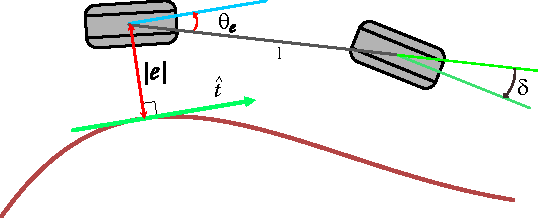
\includegraphics[width=10.5 cm]{img/path} \caption{ Feedback
        and actuator variables for the rear-wheel-based control. The magnitude
        of $e$ illustrated in red, is the error measured from the rear wheel to
        the nearest point on the path. When e > 0, the wheel is at the right of
        the path, and when e < 0 is at the left. $\theta_e$ is the
        difference between the tangent at the nearest point in the path and the
        the heading $\theta$. The output of the controller is the heading rate
        $\omega$, from which we calculate the steering angle $\delta$ of the front wheel.
}\label{fig:kinematics}    \end{figure} 

Now we explain the path tracking method described by Paden et al.
\cite{paden_survey_2016}.  This controller takes the feedback from the
rear-wheel position as Figure \ref{fig:kinematics} illustrates.  The path
(shown in red in the figure) is a continuous function with properties
described in \cite{samson1992path}, and the feedback is a function of the
nearest point on the reference path given by 

\begin{equation}\label{eq:gamma}
s(t) = \operatorname*{arg\,min}_{\gamma} \|(x_r(t),y_r(t)) - (x_{ref}(\gamma),y_{ref}(\gamma)) \|.
\end{equation}

and the tracking error vector is 

\begin{equation}\label{eq:tracking_error}
d(t) = (x_r(t),y_r(t))-(x_{ref}(s(t)),y_{ref}(s(t)))
\end{equation}

The heading error is based on a unit vector $\hat{t}$ (shown in green on Figure
\ref{fig:kinematics}) tangent to the path at $s(t)$ given by 

\begin{equation}
\hat{t} = \frac{ \left(\left.\frac{\partial x_{ref}}{\partial s} \right|_{s(t)},\left.\frac{\partial y_{ref}}{\partial s} \right|_{s(t)}\right)} 
              {\left\| \left(\frac{\partial x_{ref}(s(t))}{\partial s},\frac{\partial y_{ref}(s(t))}{\partial s}\right) \right\|},
\end{equation}

The error $e$ is the cross product of the two vectors

\begin{equation}
e = d_x \hat{t}_y - d_y \hat{t}_x
\end{equation}

The heading error uses the angle $\theta_e$ between the robot's heading vector
and $\dot(t)$

\begin{equation}
\theta_e(t) = \theta - arctan_2 \left( \frac{\partial x_{ref}(s(t))}{\partial s} , \frac{\partial y_{ref}(s(t))}{\partial s} \right)
\end{equation}



%The control law for  

%\begin{equation}
%\omega = \frac{v_r \mathcal{K}(s) \cos(\theta_e)}{1 - \mathcal{K}(s)e} - g_1(e, \theta_e,t)\theta_e - k_2v_r \frac{\sin(\theta_e)}{\theta_e}e,
%\end{equation}
%%

%Based on this model we nowfollowing a trajectory specified using cubic splines is
%described.
\subsection{Fuzzy Controller}%
    \label{sub:FuzzyControllers}

To design a fuzzy controller for the model we just described, we must decide which 
variables we are going to treat as fuzzy variables. 
First, we must consider the error ($e$), defined as the distance from the rear wheel to the
path's closest point. This error is positive if it is on the right and
negative if on the left of the path. Another input variable is the angle
$\theta_e$ defined between the heading vector and the tangent vector of the
path. This angle can also be negative or positive depending on the vehicle's
position concerning the path; the controller output is the heading rate
$\omega$, which allows us to calculate the steering angle $\delta$. The target
velocity of the robot will be constant, so we will not control (or fuzzify) the
velocity $v$ using the fuzzy controller. We will use the following simple
proportional controller instead

\begin{equation}
    a = K_p(v_{ref}-v_r).
\end{equation}

\subsubsection{Parametrizable Fuzzy Controller}
In this section, we explain the proposed a parametrizable fuzzy controller,
suitable to optimization using a bio-inspired metaheuristic. We must define 
the structure of the fuzzy controller consisting of fuzzy rules and parametrizable 
membership functions.
Extending our previous work \cite{Mancilla2021}, in which we used three MFs for each 
variable we now add two more 
membership functions to the previous fuzzy model, with the intention
of having a finer grain of control. Adding more MFs also adds more
complexity to the rules, and now we have even more parameters to tune.  Instead
of having just two values for each type of error { \tt hi } and {\tt low} we
add a middle value, represented by the { \tt medium } membership function. The
knowledge in the fuzzy rule base is now more complex than before, with 25
rules. In this case, defining the rules was not done by simply specifying a
driver's knowledge. We needed to adjust the rules by running several
simulations. The rules are presented in Table~\ref{tab:5mfRules}.

\begin{specialtable}[H]
    \caption{Proposed fuzzy rules for the basic controller with three membership functions.}\label{tab:5mfRules}
    \centering
    \begin{tabular}{lllllll}
    Rule 1:  & If $\theta_e$ is & { \tt hi\_neg}  & and $e$ is  & { \tt hi\_neg}  &	then $\omega$ is & { \tt hi\_pos}  \\
    Rule 2:  & If $\theta_e$ is & { \tt hi\_neg}  & and $e$ is	& { \tt med\_neg} &	then $\omega$ is & { \tt hi\_pos}  \\
    Rule 3:  & If $\theta_e$ is & { \tt hi\_neg}  & and $e$ is  & { \tt low}      &	then $\omega$ is & { \tt hi\_pos}  \\
    Rule 4:  & If $\theta_e$ is & { \tt hi\_neg}  & and $e$ is	& { \tt med\_pos} &	then $\omega$ is & { \tt med\_pos} \\
    Rule 5:  & If $\theta_e$ is & { \tt hi\_neg}  & and $e$ is	& { \tt hi\_pos}  &	then $\omega$ is & { \tt low}      \\
    Rule 6:  & If $\theta_e$ is & { \tt med\_neg} & and $e$ is	& { \tt hi\_neg}  &	then $\omega$ is & { \tt med\_pos} \\
    Rule 7:  & If $\theta_e$ is & { \tt med\_neg} & and $e$ is	& { \tt med\_neg} &	then $\omega$ is & { \tt med\_pos} \\
    Rule 8:  & If $\theta_e$ is & { \tt med\_neg} & and $e$ is	& { \tt low}      &	then $\omega$ is & { \tt med\_pos} \\
    Rule 9:  & If $\theta_e$ is & { \tt med\_neg} & and $e$ is	& { \tt med\_pos} &	then $\omega$ is & { \tt med\_pos} \\
    Rule 10: & If $\theta_e$ is	& { \tt med\_neg} & and $e$ is	& { \tt hi\_pos}  &	then $\omega$ is & { \tt low}      \\
    Rule 11: & If $\theta_e$ is	& { \tt low}      &	and $e$ is	& { \tt hi\_neg}  &	then $\omega$ is & { \tt hi\_pos}  \\
    Rule 12: & If $\theta_e$ is	& { \tt low}      &	and $e$ is	& { \tt med\_neg} &	then $\omega$ is & { \tt low}      \\
    Rule 13: & If $\theta_e$ is	& { \tt low}      &	and $e$ is	& { \tt low}      &	then $\omega$ is & { \tt low}      \\
    Rule 14: & If $\theta_e$ is	& { \tt low}      &	and $e$ is	& { \tt med\_pos} &	then $\omega$ is & { \tt low}      \\
    Rule 15: & If $\theta_e$ is	& { \tt low}      &	and $e$ is	& { \tt hi\_pos}  &	then $\omega$ is & { \tt hi\_neg}  \\
    Rule 16: & If $\theta_e$ is	& { \tt med\_pos} &	and $e$ is	& { \tt hi\_neg}  &	then $\omega$ is & { \tt low}      \\
    Rule 17: & If $\theta_e$ is	& { \tt med\_pos} &	and $e$ is	& { \tt med\_neg} &	then $\omega$ is & { \tt med\_neg} \\
    Rule 18: & If $\theta_e$ is	& { \tt med\_pos} &	and $e$ is	& { \tt low}      &	then $\omega$ is & { \tt med\_neg} \\
    Rule 19: & If $\theta_e$ is	& { \tt med\_pos} &	and $e$ is	& { \tt med\_pos} &	then $\omega$ is & { \tt med\_neg} \\
    Rule 20: & If $\theta_e$ is	& { \tt med\_pos} &	and $e$ is  & { \tt hi\_pos}  &	then $\omega$ is & { \tt med\_neg} \\
    Rule 21: & If $\theta_e$ is	& { \tt hi\_pos}  &	and $e$ is	& { \tt hi\_neg}  &	then $\omega$ is & { \tt low}      \\
    Rule 22: & If $\theta_e$ is	& { \tt hi\_pos}  &	and $e$ is	& { \tt med\_neg} &	then $\omega$ is & { \tt med\_neg} \\
    Rule 23: & If $\theta_e$ is	& { \tt hi\_pos}  &	and $e$ is	& { \tt low}      &	then $\omega$ is & { \tt hi\_neg}  \\
    Rule 24: & If $\theta_e$ is	& { \tt hi\_pos}  &	and $e$ is	& { \tt med\_pos} &	then $\omega$ is & { \tt hi\_neg}  \\
    Rule 25: & If $\theta_e$ is	& { \tt hi\_pos}  &	and $e$ is	& { \tt hi\_pos}  &	then $\omega$ is & { \tt hi\_neg}    
    \end{tabular}
 \end{specialtable}

The other component of a fuzzy controller are MFs, these must be defined as a parametrizable structures, 
suitable to be optimized using a metaheuristic. We describe this structures in the following section.

\subsection{Parametrizable Membership Functions}%
    \label{sec:GA}

In this section, we describe our proposed method for MFs parameter
optimization. First, we need to establish which parameters of the MFs we are
going to keep fixed and which parameters we are going to optimize. As general
rule, we keep the MFs symmetrical around zero, this means that the middle point
of the triangular MF for { \tt low} will be fixed at zero in all cases. We also
kept the extreme values of {\tt high} trapezoidal MFs, fixed at 50 and 5,
positive or negative depending on the side. We kept the parameters of $\omega$
fixed, to limit the search space. The parameters are illustrated in
Figure~\ref{tab:5mf}. In this case, we just needed ten variables to
parameterize the controller.

\begin{specialtable}[htbp]
    \small
    \caption{Ten parameter configuration for five MFs fuzzy controller.}\label{tab:5mf}
    \begin{tabular}{cccc}
    \toprule
     \textbf{Variable} & \textbf{Linguistic Value} & \textbf{MF}& \textbf{Parameters}  \\
    \midrule
    $\theta_e$ & high negative  & $\mu_{trap}$  & $[-50, -5, -b, -b+c]$     \\ 
    $\theta_e$ & medium negative& $\mu_{tria}$  & $[-d-e, -d, -d+e]$     \\ 
    $\theta_e$ & low            & $\mu_{tria}$  & $[-a, 0, a]$     \\ 
    $\theta_e$ & medium positive& $\mu_{tria}$  & $[-d-e, d, d+e]$     \\ 
    $\theta_e$ & high positive  & $\mu_{trap}$  & $[b-c, b, 5, 50]$ \\

    \midrule
    $error$ & high negative  & $\mu_{trap}$  & $[-50, -5, -g, -g+h]$     \\ 
    $error$ & medium negative& $\mu_{tria}$  & $[-i-j, -i, -i+j]$     \\ 
    $error$ & low            & $\mu_{tria}$  & $[-f, 0, f]$     \\ 
    $error$ & medium positive& $\mu_{tria}$  & $[-i-j, i, i+j]$     \\ 
    $error$ & high positive  & $\mu_{trap}$  & $[g-h, g, 5, 50]$ \\

    \midrule
    $\omega$ & high negative  & $\mu_{trap}$  & $[-50, -5, -1, -0.5]$     \\ 
    $\omega$ & medium negative& $\mu_{tria}$  & $[-1, -0.5, 0]$     \\ 
    $\omega$ & low            & $\mu_{tria}$  & $[-0.5, 0, 0.5]$     \\ 
    $\omega$ & medium positive& $\mu_{tria}$  & $[0, 0.5,1]$     \\ 
    $\omega$ & high positive  & $\mu_{trap}$  & $[0.5, 1 ,5, 50]$     \\ 
    \bottomrule
\end{tabular}
\end{specialtable}

Another essential aspect to consider when tuning the above parameters is the
range of values that each parameter can have. Normally, we keep all the
parameters in the same range when using a population-based metaheuristic. In
our previous work \cite{Mancilla2021}, we compared two ranges  
$[0,1]$ and $[0,2]$ our experiments showed better results with the
narrower range, so we selected the same configuration for the three MFs
controllers for this work. In this work, we propose a simple technique to
change the tuning ranges for the MFs while keeping the adjustable parameters in
the same range of values $[0,1]$. We define different ranges for the input
variables and normalize the values before they are passed to the membership
functions. We can treat this as an aperture factor, now each parameter of 
a MF can have a distinct range, while keeping the parameters or be optimized 
fixed on $[0,1]$. We defined from our experience the range for each parameter, these 
are shown in Table~\ref{tab:factor}.

\begin{specialtable}[H] 
\small
\caption{Ranges defined for each parameter for the 5MF controller.}\label{tab:factor}
\begin{tabular}{clcl}
\toprule
\textbf{Parameter}	& \textbf{Range}& \textbf{Parameter} & \textbf{Range}\\
\midrule
a & [0,1]			& f & [0, 1]\\
b & [0.5,2]			& g & [0.5, 2]\\
c & [0,2]			& h & [0, 2]\\
d & [0.5,1.5]		& i & [0.5,1.5]\\
e & [0,1]			& j & [0, 1]\\
\bottomrule
\end{tabular}
\end{specialtable}

\subsubsection{Optimization Problem Formulation}

An optimization procedure is needed to tune the parameters of the 
membership functions in order to generate a fuzzy controller that maintains 
a low positional error over a desired path. The optimization problem 
can be defined as searching for the parameter vector $x^{mf}$ that defines the membership functions 
which minimize  the error. This can be defined as: 

\begin{equation}
    \operatorname*{arg\,min}_{x^{mf}} \{ FC_{error}\}
\end{equation}

where the fitness function $FC_error$ is the average RMSE of three simulations:

\begin{equation}
  FC_{error} = \frac{1}{3} \sum_{k=1}^3 rmse(FC(x^{mf}), s_k, t_{max}) 
\end{equation}

in which $k$ is the number of paths $s_k$. A simulation consists of running a control problem as 
defined in Section~\ref{sec:kinematic} in which the control is
performed by the fuzzy controller $FC(x^{mf})$ with membership functions
defined by $x^{mf}$. The constant $t_{max}$ is the number of cycles executed in one simulation.
As described before, the controller objective is to minimize the tracking error, 
to obtain the RMSE we can use the tracking error vector defined in Equation~\ref{eq:tracking_error}:

\begin{equation}\label{eq:tracking_error}
 rmse = \sqrt{\frac{\sum_{t=1}^{t_{max}} (x_r(t),y_r(t))-(x_{ref}(s_k(t)),y_{ref}(s_k(t)))^2}{t_{max}}}
\end{equation}

The vector $x^{mf}$ defines the parameters of the membership functions defined in Table~\ref{tab:5mf} 
and the knowledge base in Table~\ref{tab:5mfRules}: 

\begin{equation}\label{eq:mfs}
 x^{mf} = \{x_1^a, x_2^b, x_3^c, x_4^d, x_5^e, x_6^f, x_7^g, x_8^h, x_9^i, x_{10}^j\}
\end{equation}

The range of all parameters is between 1 and 0: 

\begin{equation}\label{eq:mfs}
  0 \leq x_i \leq 1
\end{equation}


\subsubsection{Metaheuristic Optimization Procedure}\label{sec:GAO}

In general, a population-based metaheuristic, needs to evaluate the fitness of
each candidate solution (also called individuals) in its population. This
process is illustrated in Figure~\ref{fig:ga}. Each candidate solution is
represented by a vector $x^{mf}$, here implemented as a list of objects of type {
\tt float }. To evaluate each solution, we need to generate an instance of the
fuzzy controller. Once created, the fuzzy controller is passed as a
parameter, together with the paths the mobile robot will follow. The output of
the simulations is the RMSE of the accumulated errors $e$ obtained during the
simulations. We consider this measure as the fitness of the candidate solution.

\begin{figure}[H]
\centering
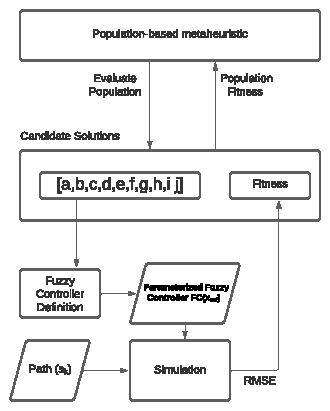
\includegraphics[width=9 cm]{img/ga}
\caption{
For each candidate solution in the population, a controller is created with the
parameters, this controller is then tested by running one or more simulations.
The RMSE of the tracking is considered as the fitness for that particular
candidate solution. This process is repeated for each member of the
population.
}\label{fig:ga}
\end{figure} 

In our previous work \cite{Mancilla2021} we used a GA to evolve the controllers 
using a single path; we noticed that this could lead to over-training. Similar to what
happens in supervised learning algorithms, the controller found by the GA could
be specialized only to the path used for its evolution. We found that the
controller with only three MFs could follow new unseen paths, but this was not
the case for the five MFs controller. It is well known that in rule-based
learning, adding more rules can harm the capacity to generalize to unseen
problems \cite{tan2016introduction}. Noticing this, we added a list of three
paths to evaluate the fitness for the experiments, which is the average RMSE
of the three simulations. We ran experiments with one and three paths. We
defined each path using cubic splines over a list of coordinates; this is a
common approach in the literature \cite{zhang2013cubic}. The paths and the
parameters to define them are shown in Table~\ref{tab:routes}. The first path
was used on previous work and was taken from the library of
\cite{sakai_pythonrobotics_2018}, this path starts with a very narrow curve to
the left that is difficult for controllers to follow, but it remains
differentiable throughout the path, we call this path ``M''. The other paths
are called ``A'' and ``S'' and have smoother curves, with long straight
segments and different curvatures. All paths have seven anchor points for the
cubic spline.

\begin{specialtable}[H] 
\small
\caption{Tracks used for fitness evaluation, they are defined by cubic splines with the parameters shown below each plot.\label{tab:routes}}
\begin{tabular}{lll}
\toprule
\multicolumn{1}{c}{\textbf{Track M}}		& \multicolumn{1}{c}{\textbf{Track A}}& \multicolumn{1}{c}{\textbf{Track S}}\\
\midrule
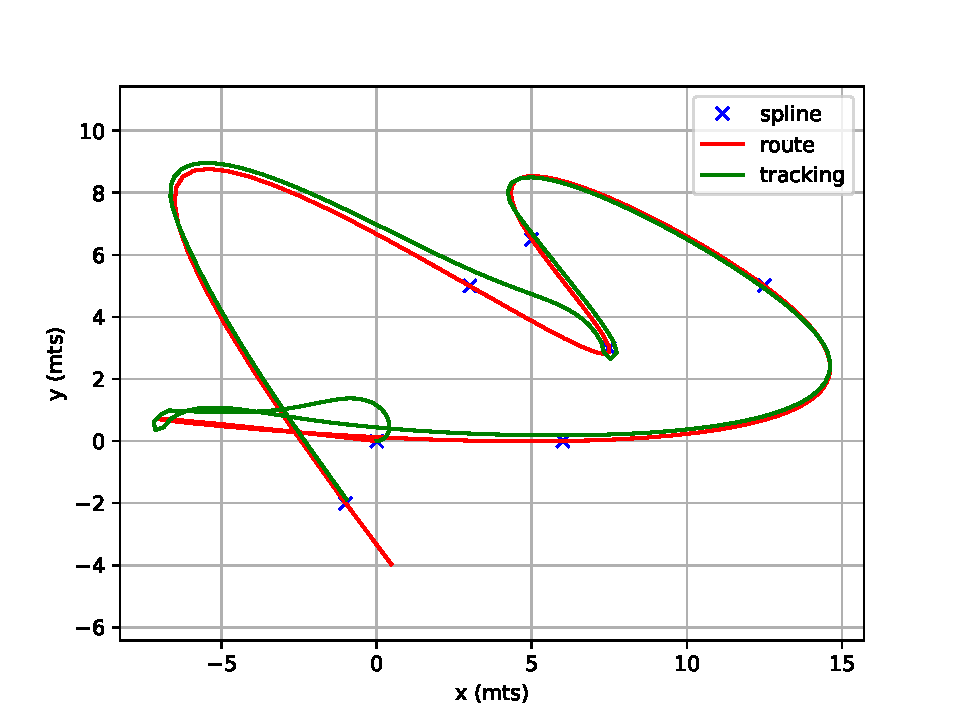
\includegraphics[scale=0.23]{img/M.pdf}& 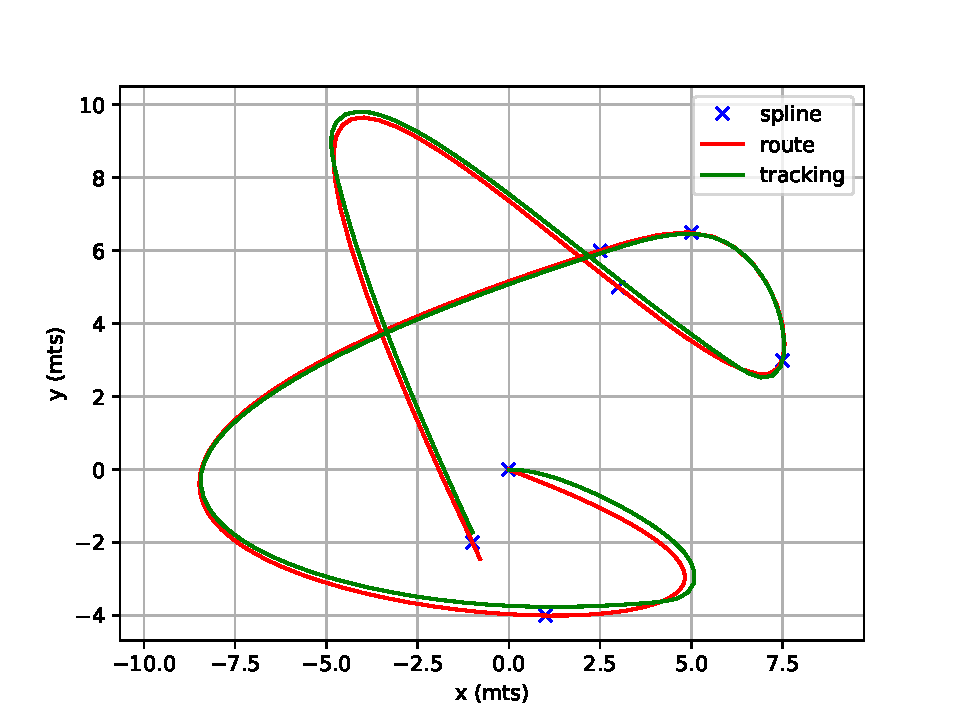
\includegraphics[scale=0.23]{img/A.pdf} & 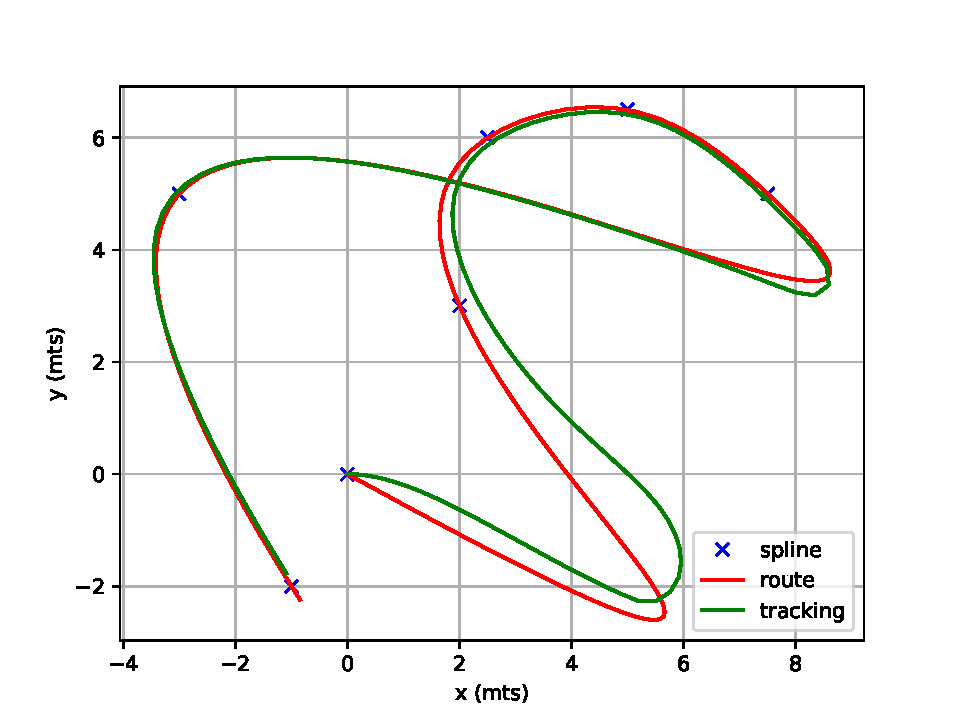
\includegraphics[scale=0.23]{img/S.pdf}\\
  $ax=[0,6,12,5,7.5,3,-1]$	&$ax = [0, 1, 2.5, 5, 7.5, 3, -1] $& $ ax = [0, 2, 2.5, 5, 7.5, -3, -1]$\\
  $ay = [0, 0,  5, 6.5, 3, 5, -2]  $	&$ay = [0, -4, 6, 6.5, 3, 5, -2] $& $ ay = [0, 3, 6, 6.5, 5, 5, -2] $\\
\bottomrule
\end{tabular}
\end{specialtable}

\subsubsection{Complexity of the Optimization Procedure}
 
The computational complexity of the optimization procedure described earlier,
depends mostly on the evaluation of the fitness function. In this case, is
difficult to estimate the cost of each simulation step because it depends on an
ordinary differential equation solver (ODEInt), in particular this is a
multi-step solver (lsode) and the number of iterations changes depending on the
initial conditions. Moreover, in order to calculate the current nearest point
to the path as described in Equation~\ref{eq:gamma}, there is a local
optimization procedure to find $\gamma$ to establish this nearest point
$(x_ref(\gamma),y_ref(\gamma))$.j Nevertheless, we can consider the cost of the
function evaluation as domain dependent and with a high order complexity of at
least $\mathcal{n^3}$. Because of this, normally the number of function
evaluations needed to find a solution considered when establishing the
performance of a metaheuristic algorithm. 

On the side of population-based algorithm, and in particular all the algorithms
that we tested on this paper, follow the same procedure: randomly initialize
the population, this has a $\mathcal{O}(n)$ complexity, with $n$ the population
size (the number of candidate solutions).  After the evaluation, there is a
step for updating the solution the complexity for this is normally
$\mathcal{O}(m*n)+\mathcal{O}(m*n*l)$ $m$ is the number of iterations and $l$
the number or parameters in the fitness function. Some algorithm add a step for
keeping only the generated solutions if the new fitness is better, this has an
additional cost of $\mathcal{O}(n)$, finally there are algorithms that order
the population by fitness after every iteration, this adds a complexity of
$\mathcal{O}(nlog{}n)$.


\subsubsection{Experimental Setup} % (fold)
\label{sub:setup}

In this section, we compare the parameter optimization procedure proposed in 
the previous section, using the following algorithms:

\begin{enumerate}
    \item Genetic Algorithm (GA) \cite{holland1992genetic} 
    \item Particle Swarm Optimization (PSO) \cite{kennedy2006swarm} 
    \item Aquila Optimization (AO) \cite{abualigah2021aquila} 
    \item Grey Wolf Optimizer (GWO) \cite{mirjalili2014grey} 
    \item Arithmetic Optimization Algorithm (AOA) \cite{abualigah2021arithmetic} 
    \item Harmony Search (HS) \cite{geem2001new} 
\end{enumerate}

All algorithms have the same population size of 50, and the number of iterations 
was set at 30, from this values, the total number of function evaluations is 1000. 
The parameters of the comparative algorithms is shown in Table~\ref{tab:alg_params}.

\begin{specialtable}[H] 
\small
\caption{Parameter values for the algorithms compared}\label{tab:alg_params}
\begin{tabular}{lll}
\toprule
\textbf{Algorithm} & \textbf{Parameter}	& \textbf{Value}\\
\midrule
GA & Selection & Tournament Selection (k =3)  \\
& Mutation  & Gaussian ($\mu=0.0$ and $\sigma=0.2$)  \\
& Mutation probability  &  0.3 \\
& Crossover  & One point crossover (probability = 0.7)   \\
\midrule
PSO & Topology & Fully connected  \\
& Speed limit& Min=-0.25,Max=0.25   \\
& Cognitive and Social constants & $C_1=2,C_2=2$   \\
\midrule
AO & $\alpha$ & 0.1  \\
& $\delta$ & 0.1  \\
\midrule
GWO & Convergence parameter (a)& Linearly decreased from 2 to 0  \\
\midrule
AOA & $\alpha$ & 5  \\
& $\mu$ & 0.5  \\
\midrule
HS & HMConsidering Rate (HMCR) & 0.95  \\
& Pitch Adjusting Rate & 0.05  \\
\bottomrule
\end{tabular}
\end{specialtable}

%The population si
%we implemented the algorithm in python using the deap \cite{fortin_deap_2012}
%library for the ga implementation. we used the scikit-fuzzy
%\footnote{https://github.com/scikit-fuzzy/scikit-fuzzy} library to code the
%fuzzy inference  systems. finally, we modified a fork of the pythonrobotics
%repository \cite{sakai_pythonrobotics_2018}, adding the odeint library from the
%scipy package \footnote{https://github.com/scipy/scipy} to integrate the system
%of ordinary equations.
%all experiments ran with the same parameters for the ga. the only obvious
%difference was the size of the chromosomes because this is the same as the
%number of parameters we need to optimize. as we mentioned earlier, we proposed
%two controllers, one with three membership functions; we are going to call this
%controller 3mf, and the other controller 5mf because it has five membership
%functions. for details on these controllers, see
%section~\ref{sub:fuzzycontrollers}.  after several preliminary experiments, we
%settled for a configuration with a population size of 50 with 20 generations.
%We used single-point crossover with $0.3$ probability.  We opted for tournament
%selection with a tournament size of three. For mutation, and because we are
%using continuous values, we selected a Gaussian mutation with $\mu=0.0$ and
%$\sigma=0.2$. Finally, the probability for each gene to be mutated was $0.2$.
The fitness function returns the RMSE of the simulation as mentioned earlier,
but to economize the
computational resources, while the simulations were running, we interrupted
those simulations where the robot was clearly out of the path or did not
finish near the final point of the path. In these cases, we assigned a very
low fitness (we want to minimize the error) of 5000 to the first case and 2000
to the second.  

As the basis for comparison, we compare or results against the controller in
\cite{paden_survey_2016}, with the following control law defined as 

\begin{equation}\label{eq:controller}
\omega = \frac{v_r \mathcal{K}(s) \cos(\theta_e)}{1 - \mathcal{K}(s)e} -
  (k_{\theta}|v_r|)\theta_e - \left( k_ev_r \frac{\sin(\theta_e)}{\theta_e}\right) e,
\end{equation}

the parameters of the simulations and the canonical controller we are comparing
against are summarized in Table~\ref{tab:sim_params}.

\begin{specialtable}[H] 
\small
\caption{Simulation and controller parameters.}\label{tab:sim_params}
\begin{tabular}{ll}
\toprule
\textbf{Parameter}	& \textbf{Value}\\
\midrule
Wheel-base & $l=2.5$		\\
Steering limit & $|\delta|\le \frac{\pi}{4}$	\\
Initial configuration & $x_r(0),y_r(0),\theta(0)= (0,0,0)$\\
Velocity controller configuration & $K_p=1, v(0)=0, a(0)=0$\\
Target velocity & $v_r=\frac{10}{3}$\\
Maximum time & 50 \\ 
Control law parameters&$k_e=0.3, k_{\theta}=1.0$\\ 
\bottomrule
\end{tabular}
\end{specialtable}

We ran the experiments on a Desktop PC with AMD Ryzen 9 3900x 12-core processor
with 24 threads and 48 GB RAM with Ubuntu Linux 21.04, and Python 3.7.5 code.
Code and data can be found in the following GitHub repository
\url{https://github.com/mariosky/fuzzy-control}.

We compared the algorithms using the mean, median and standard deviation of the RMSE 
of 30 algorithm executions. Moreover, we performed a Wilcoxon rank-sum test between algorithms 
for performance comparison. 

% subsubsection (?4:_:\lGA)(?4:_:\l)(?4:_:\limplementation) (end)


%%%%%%%%%%%%%%%%%%%%%%%%%%%%%%%%%%%%%%%%%
\section{Results}\label{Results}

This section shows the results of running the optimization of parameters for
the controller described in the previous sections, with the average RMSE of
three paths to establish the fitness. The descriptive statistics of these
results are shown in Table~\ref{tab:statistics}.  As expected, and because the
optimization is non-deterministic, there are a few outliers at both extremes of
the performance. In particular, outliers are presented on the GA algorithm with
RMSE = 0.18205, and the AOA algorithm with RMSE = 0.7978. The PSO algorithm
obtained the lower RMSE average (0.00546) and the best controller (0.00158) and
AOA with median of (0.00523). 

\begin{specialtable}[H] 
\small
\caption{Descriptive statistics (n=30) results for algorithms with an evaluation
    with three paths.}\label{tab:statistics}
\begin{tabular}{llllll}
\toprule
\textbf{Algorithm} & \textbf{Average }	& \textbf{Standard } &\textbf{Median} & \textbf{Min} & \textbf{Max}\\
                   & \textbf{RMSE}	    & \textbf{ Deviation}&                &              &            \\
\midrule
GA                  &  0.01564           & 0.03163              & 0.00918     &   0.00574    &  0.18205   \\
PSO                 &  \textbf{0.00546}  & 0.00202              & 0.00536     &   \textbf{0.00158}    &  0.00102   \\
AO                  &  0.00695           & 0.00210              & 0.00696     &   0.00355    &  0.01407   \\
GWO                 &  0.00617           & \textbf{0.00170}     & 0.00643     &   0.00315    &  0.00849   \\
AOA                 &  0.03413           & 0.14403              & \textbf{0.00198} & 0.00198 &  \textbf{0.79780}   \\
HS                  &  0.00774           & 0.00273              & 0.00740     &   0.00320    &  0.01454   \\
\bottomrule
\end{tabular}
\end{specialtable}

In Figure~\ref{fig:boxplot}, we can see that the GA algorithm has the worst median and overall results,
while the rest algorithms obtained competitive results.

\begin{figure}[H]
\centering
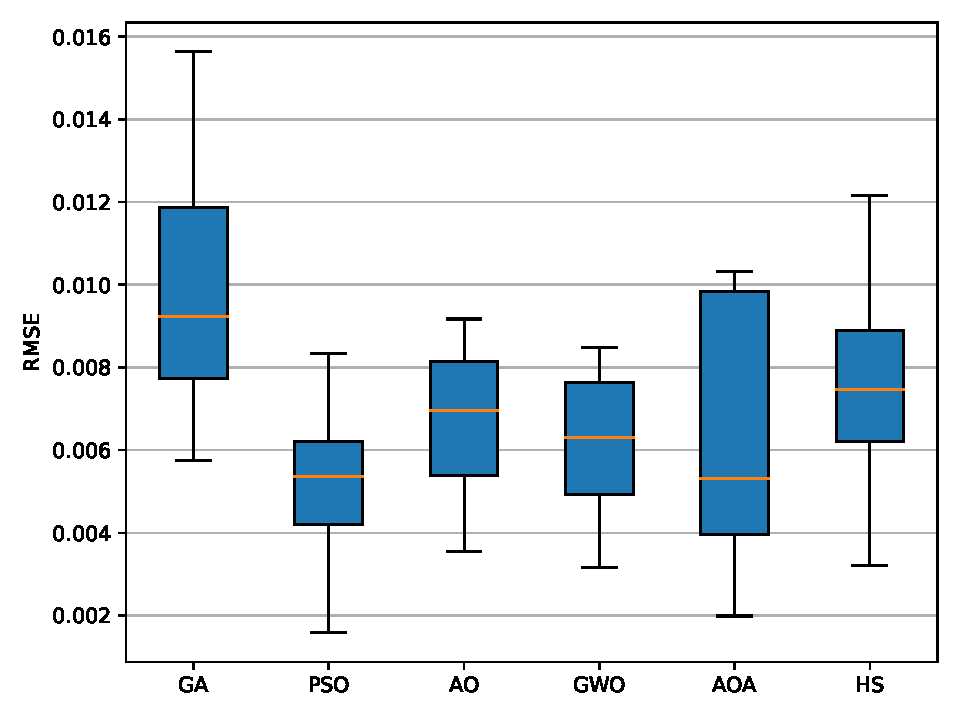
\includegraphics[width=9 cm]{img/boxplot}
\caption{
Boxplot showing the results of 30 experiments, with outliers filtered in order to 
show the plot at a larger scale.
}\label{fig:boxplot}
\end{figure}

Table~\ref{tab:wilcoxon} gives the results of the Wilcoxon rank-sum test with
an alternative hypothesis $H_1$ comparing if the algorithm in each row has a
lower median than the algorithm on each column with a significance level at
$\alpha = 0.05$. Results with a p-value lower than 0.05 are shown in bold.
Among the six algorithms, the PSO algorithm outperformed the GA, AO, GWO and HS
algorithms. The GA algorithm was outperformed by all the algorithms. The AOA
algorithm was not outperformed by any algorithm with enough statistical
significance. The GWO algorithm beat the HS algorithm, making it the second
best in number of wins.  Nevertheless, in general, most algorithms (PSO, AO,
AOA and GWO) achieved good results.

\begin{specialtable}[H] 
\small
\centering
\caption{Wilcoxon rank-sum test between algorithms, showing p-values for $H_1:A<B$}\label{tab:wilcoxon} 
\begin{tabular}{ccccccc}
\toprule 
    & GA       & PSO      & AO       & GWO      & AOA      & HS       \\
\midrule
GA  &          & 1.00E+00 & 1.00E+00 & 1.00E+00 & 9.99E-01 & 9.99E-01 \\
\midrule
PSO & \textbf{6.44E-09} &          & \textbf{2.23E-03} & \textbf{3.80E-02} & 1.73E-01 & \textbf{9.54E-05} \\
\midrule
AO  & \textbf{1.20E-05} & 9.98E-01 &          & 9.22E-01 & 7.76E-01 & 1.33E-01 \\
\midrule
GWO & \textbf{1.19E-07} & 9.63E-01 & 7.96E-02 &          & 4.80E-01 & \textbf{1.31E-02} \\
\midrule
AOA & \textbf{1.02E-03} & 8.31E-01 & 2.28E-01 & 5.25E-01 &          & 1.10E-01 \\
\midrule
HS  & \textbf{1.24E-03} & 1.00E+00 & 8.70E-01 & 9.87E-01 & 8.92E-01 &          \\
\bottomrule
\end{tabular}
\end{specialtable}

To present a qualitative comparison, we selected two of the best controllers
found in the 30 experiments,  one from the best algorithm (PSO) and the other
from the worst (GA), and then compare them against the baseline, a controller
using the control law in Equation~\ref{eq:controller}. This results are
presented in Table~\ref{tab:rmse}. We can see that even the fuzzy controller
optimized with the GA outperformed the control law in two paths. The results 
of the PSO are highly competitive against the baseline.

\begin{specialtable}[H] 
\small
\caption{RMSE of the best controllers in all three paths.}\label{tab:rmse}
\begin{tabular}{llll}
\toprule
\textbf{Path}	& \textbf{Control } &\textbf{PSO}	& \textbf{GA}\\
	& \textbf{law} & & \\
\midrule
Path M & 2.003 & \textbf{0.00217} & 0.00396 \\
Path A & 0.014 & \textbf{0.00168} & 0.00575 \\
Path S & 0.521 & \textbf{0.00195} & 0.00845 \\
\bottomrule
\end{tabular}
\end{specialtable}

When we observe the optimized MFs for both controllers, GA in
Figure~\ref{fig:3mf} and PSO in Figure~\ref{fig:5mf}, we can see that they are
similar on the \texttt{low} and \texttt{high} MFS, for both the $\theta_r$ and
$e$. There is a noticeable difference however in the high negative and low
negative MFs. in each of them both variables are very similar.  We can also see
that the MFs of $\omega$ remain fixed on both, this is because we kept those
parameters fixed. The best parameters found from all algorithms are shown in
Table~\ref{tab:params}.

\begin{specialtable}[H] 
\small
\caption{RMSE of the best controllers in all three paths.}\label{tab:params}
\begin{tabular}{ll}
\toprule
\textbf{Algorithm}	& \textbf{Parameter Vector}\\ 
\midrule
GA & \\
PSO & [0.78, 0.48, 0.43, 0.69, 0.88, 0.96, -0.13, 0.36, 0.60, 0.77]\\
AO & [0.71, 0.41, 0.44, 0.22, 0.52, 0.61, 0.12, 0.36, 0.50, 0.18]\\
GWO & [0.74, 0.46, 0.49, 0.59, 0.40, 0.40, 0.11, 0.36, 0.30, 0.53]\\
AOA & [1.0, -0.36, 0.37, 0.83, -0.47, 1.0, 0.00, 0.27, 0.27, 0.92]\\
HS & [0.96, 0.65, 0.55, 0.13, 0.62, 0.56, 0.12, 0.36, 0.96, 0.96]\\
\bottomrule
\end{tabular}
\end{specialtable}

We now show a plot of the paths and the robot's movement following the path.
First, we have the path ``M'' (see Figure~\ref{fig:3RutasM}), in which all
controllers have problems at the beginning with a curve that is very sharp to
the left and then a sharp U-turn to go back to the start.  We can see that the
Control law follows the path with less zig-zag than the GA and PSO controllers, that
keep the tracking closer to the path but with noticeable zig-zagging.

The plots in Figure~\ref{fig:3RutasA} show the ``A'' path. This time all
controllers closely follow the path. Again controller GA has a noticeable
zig-zagging but manages to have a lower RMSE than the Control law.

The results of Figure~\ref{fig:3RutasS} highlight the overall behavior of the
three controllers on path ``S''. The control law takes more time to reach the path when it
deviates from the reference because it has smoother steering, but once it is
over the path, $e$ does not increase.  That is by design because one of the
conditions is that a small initial tracking error will remain small. On the
other hand controller PSO, does not deviate much from the reference, and has a
smoother control than the GA.

\end{paracol}
\begin{figure}[H]
    \widefigure
     \centering
    \subfigure[Optimized membership functions of the best controller optimized with the PSO algorithm.]{\label{fig:3mf}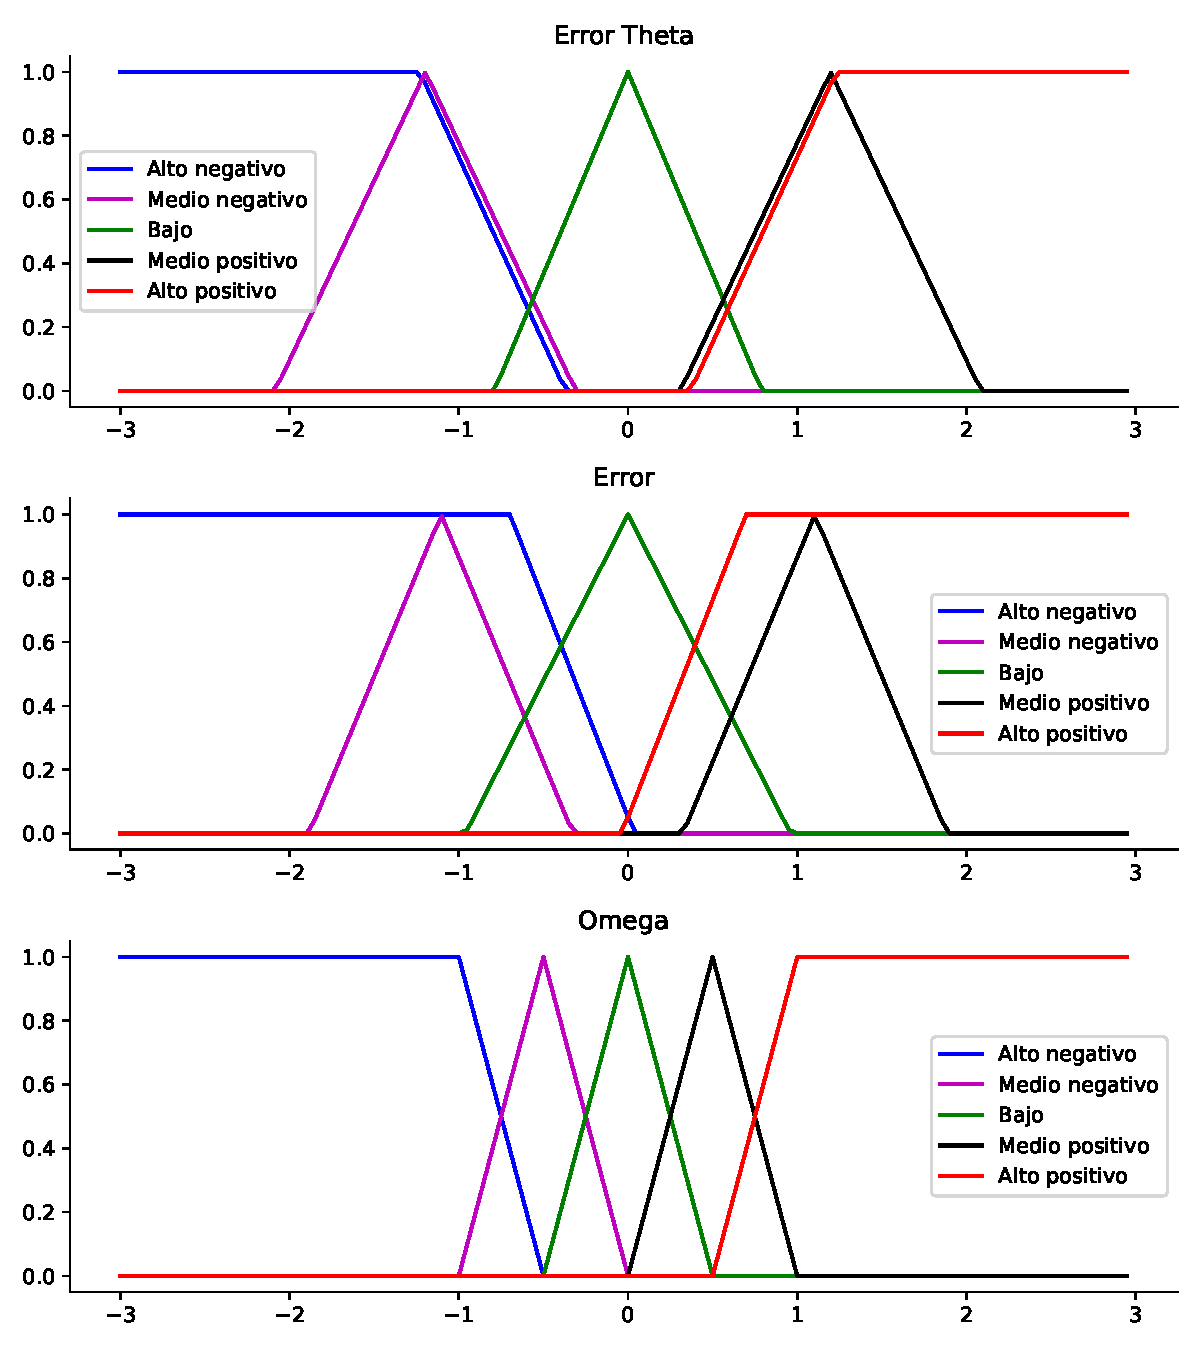
\includegraphics[width=90mm]{img/psoFIS.pdf}}
    \subfigure[Optimized membership functions of the best controller optimized with the GA algorithm.]{\label{fig:5mf}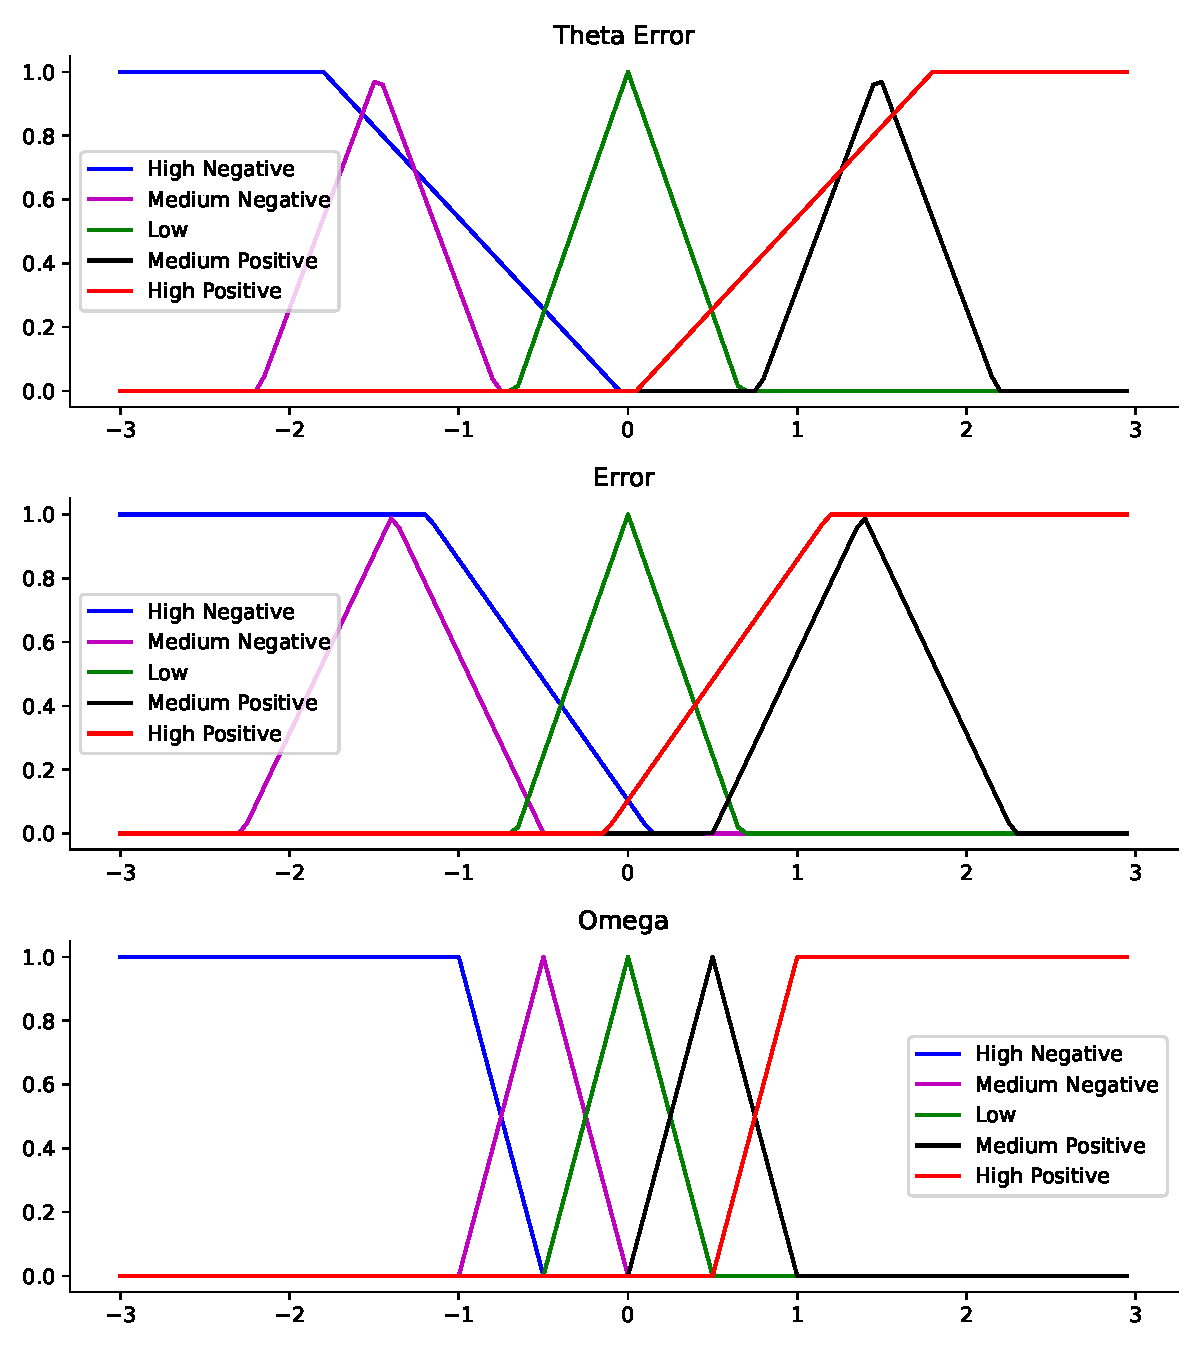
\includegraphics[width=90mm]{img/3r5fmR.pdf}}
     \caption{Optimized membership functions with PSO and GA algorithms, parameters are shown in Table~\ref{tab:params}.}
        \label{fig:MFs}
\end{figure}
\begin{paracol}{2}
\linenumbers
\switchcolumn



\end{paracol}
\begin{figure}[H]
    \widefigure
     \centering
    \subfigure[Control law]{\label{fig:compM}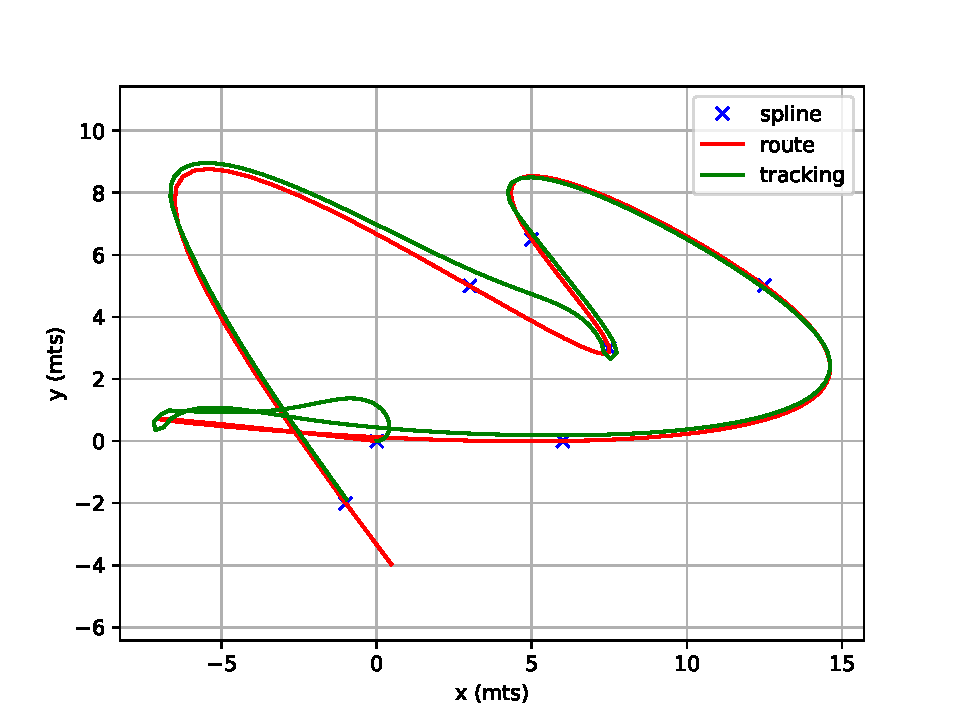
\includegraphics[width=60mm]{img/M.pdf}}
    \subfigure[PSO]{\label{fig:comp3MF}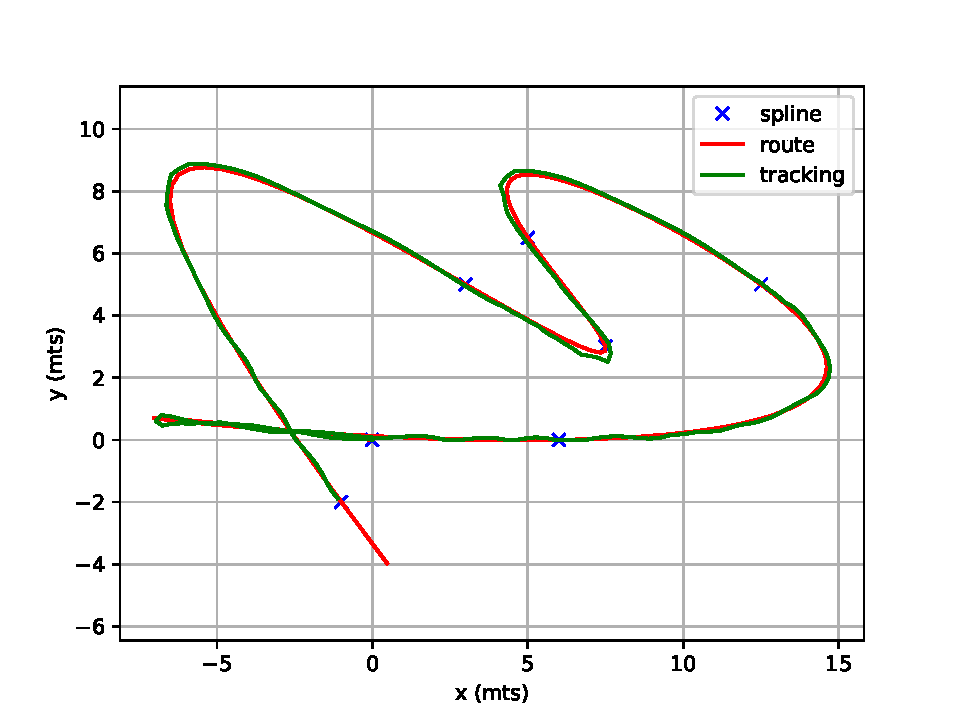
\includegraphics[width=60mm]{img/psoM.pdf}}
    \subfigure[GA]{\label{fig:comp5FM}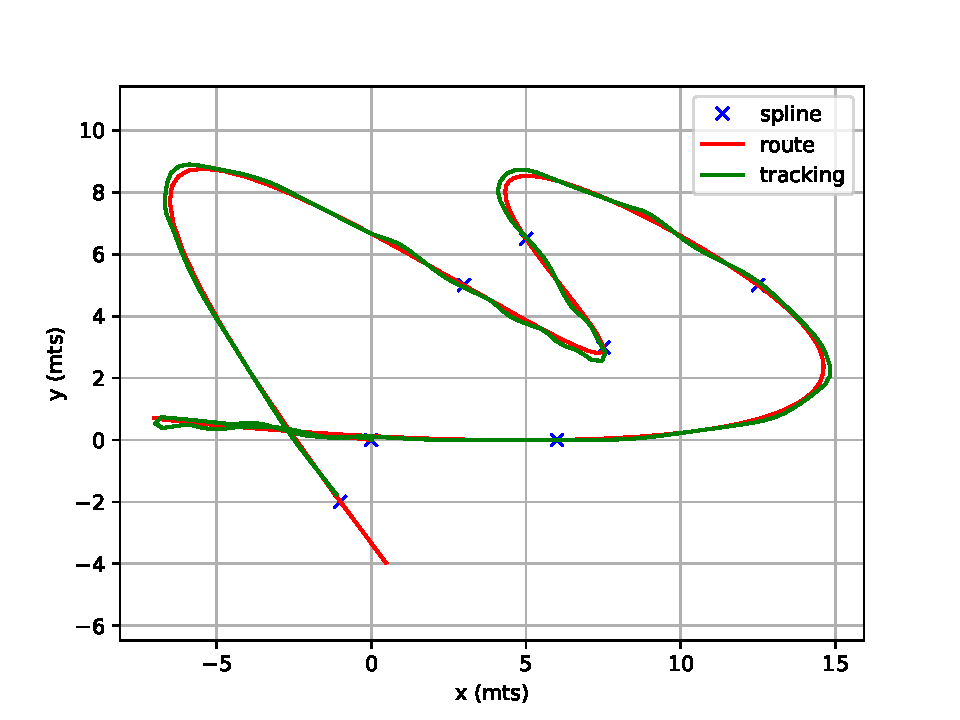
\includegraphics[width=60mm]{img/3r5fmM.pdf}}
     \caption{Plot for the best simulations on Track M.}
        \label{fig:3RutasM}
\end{figure}
\begin{paracol}{2}
\linenumbers
\switchcolumn









%%%%%%%%%%%%%%%%%%%%%%%%%%%%%%%%%%%%%%%%%%
\section{Discussion}\label{Discussion}

In this paper, we have proposed a method using a GA metaheuristic for evolving
fuzzy controllers by optimizing its membership function's parameters.  The
fuzzy controller, aimed at autonomous path tracking, using rear-wheel feedback,
was optimized by running simulations and measuring the RMSE of the distance
between the robot's position and a reference path. We compared two controllers
with distinct fuzzy inference systems, using three MFs for each variable and a
second with five MFs. Adding more MFs and, consequently, more fuzzy rules added
more complexity to the knowledge base, adding more granularity to the
representation.  We have shown that this change improved the control in terms
of RMSE, although needing more computational resources on the evolutionary
phase. With additional experiments, we have shown that by adding additional
simulations to establish the quality of candidate solutions, during the
evolution, the generated controllers have better performance than those evolved
with just one simulation.

When comparing the controllers, we found that some solutions had undesired yaw
oscillation while keeping a low RMSE; this is a crucial aspect to be considered
in future work. We can consider including a damping module or an evaluation
metric that negatively weights this kind of oscillation. We can even include a
fuzzy variable to the controller; in comparison, the control law also uses the
curvature of the path $\mathcal{K}(s)$ as a variable for determining $\omega$.
Perhaps we need to treat the evolutionary optimization of fuzzy controllers as
a supervised learning task. The assessment of the quality of solutions needs to
consider other metrics as part of the desired control properties, such as
oscillation, overshoot, and generalization capabilities.

\end{paracol}
\begin{figure}[H]
    \widefigure
     \centering
    \subfigure[Control law]{\label{fig:compA}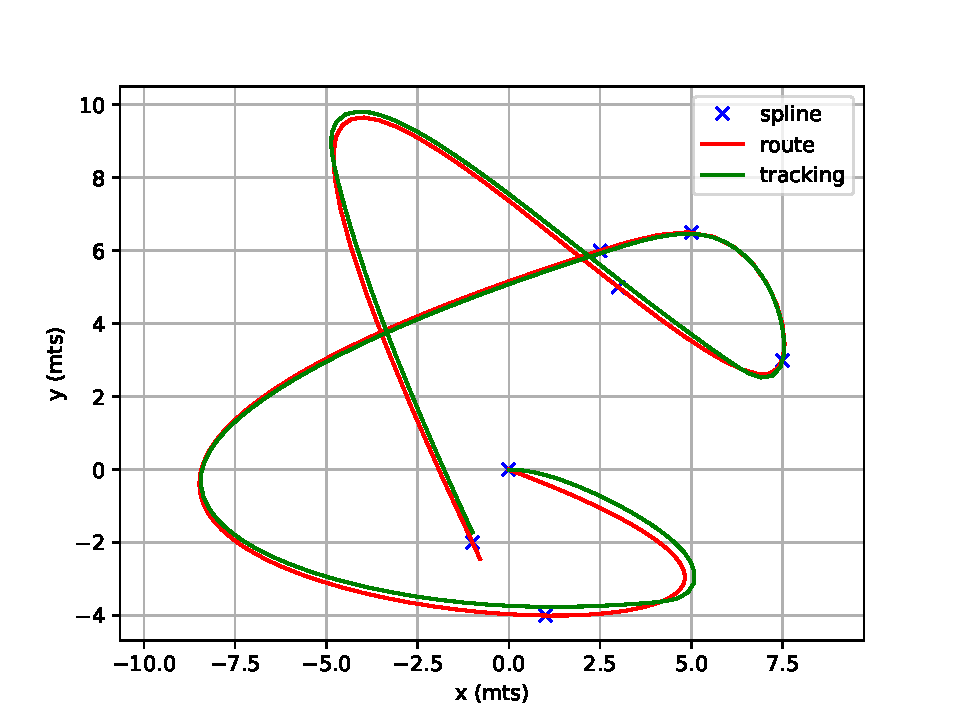
\includegraphics[width=60mm]{img/A.pdf}}
    \subfigure[PSO]{\label{fig:compA3MF}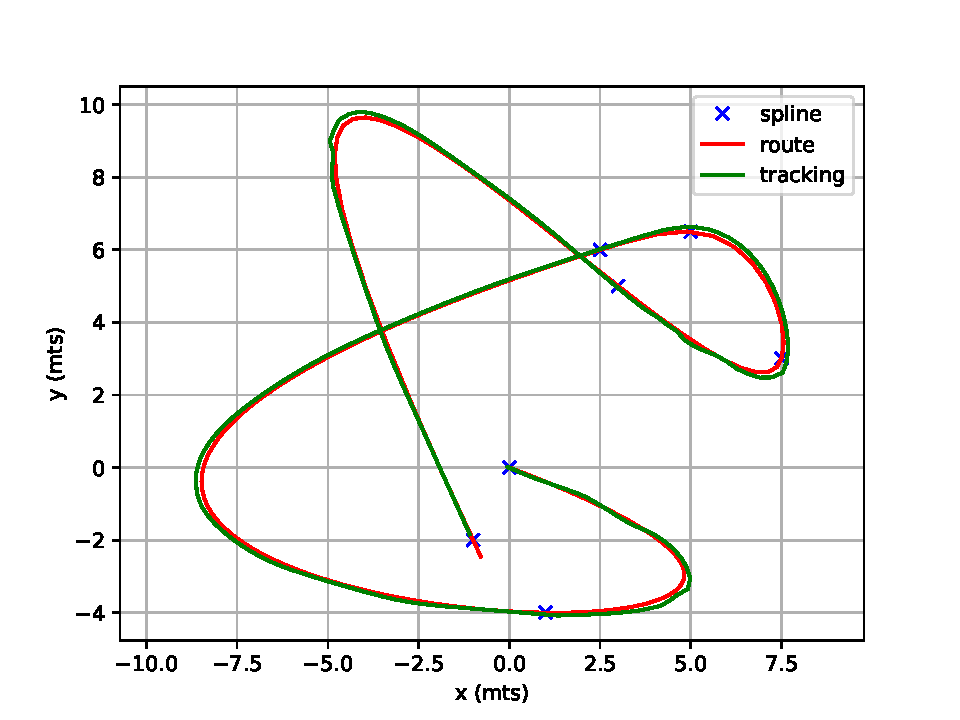
\includegraphics[width=60mm]{img/psoA.pdf}}
    \subfigure[GA]{\label{fig:compA5FM}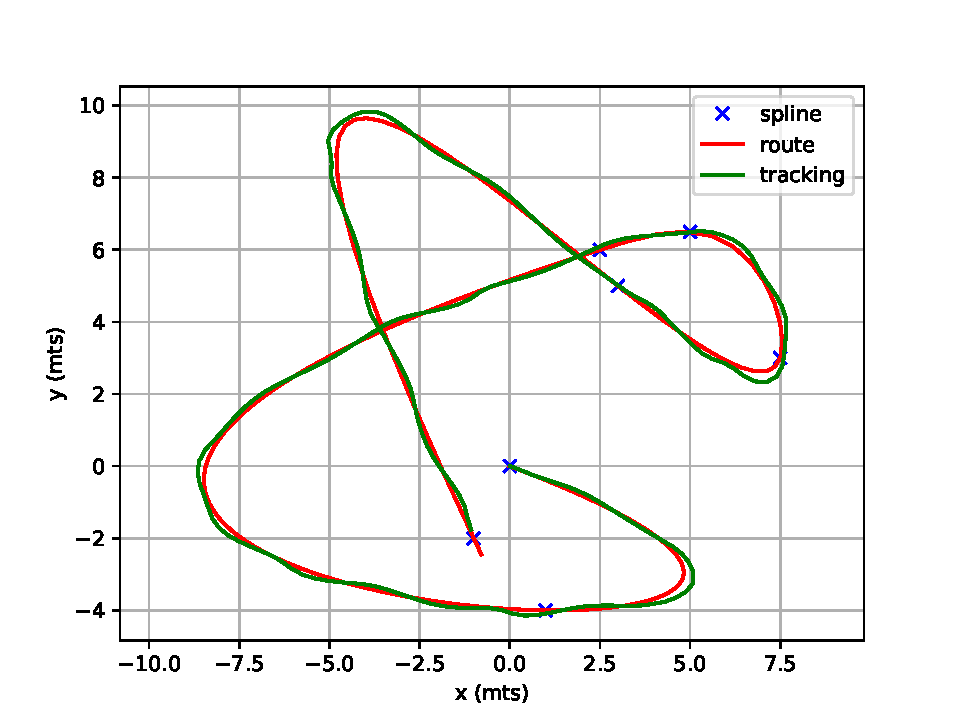
\includegraphics[width=60mm]{img/3r5fmA.pdf}}
     \caption{Plot for the best simulations on Track A.}
        \label{fig:3RutasA}
\end{figure}
\begin{paracol}{2}
\linenumbers
\switchcolumn

\end{paracol}
\begin{figure}[H]
    \widefigure
     \centering
    \subfigure[Control law]{\label{fig:compA}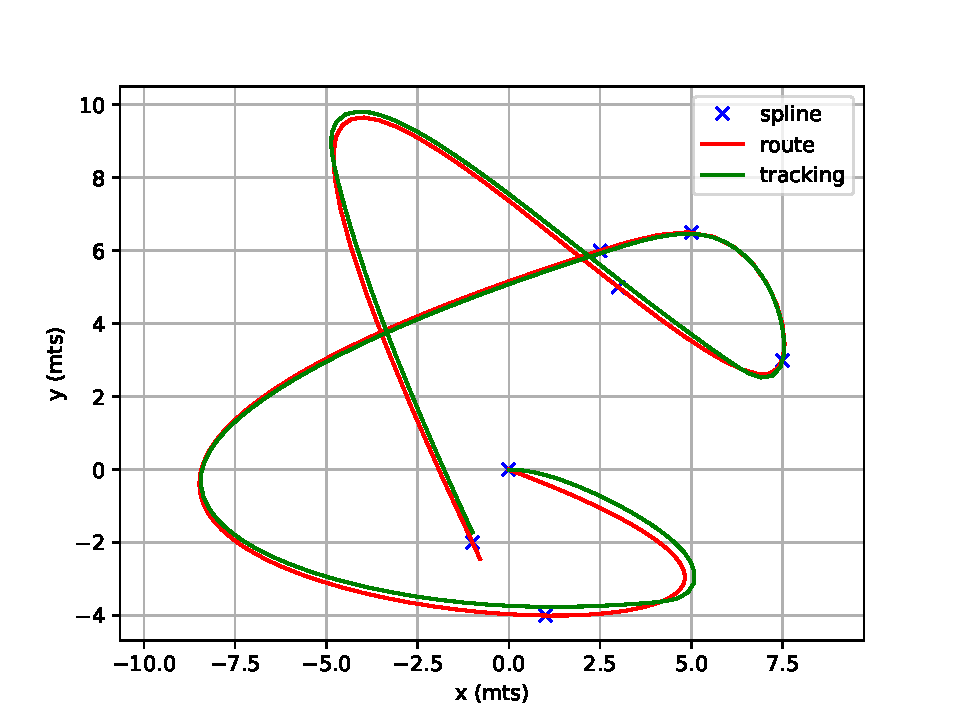
\includegraphics[width=60mm]{img/A.pdf}}
    \subfigure[PSO]{\label{fig:compA3MF}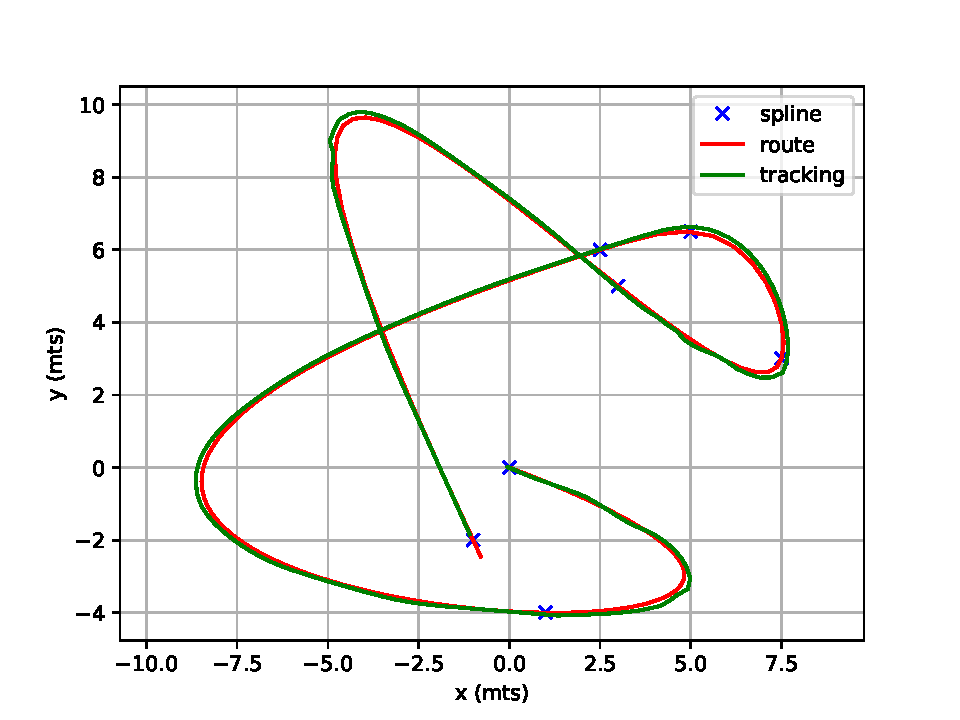
\includegraphics[width=60mm]{img/psoA.pdf}}
    \subfigure[GA]{\label{fig:compA5FM}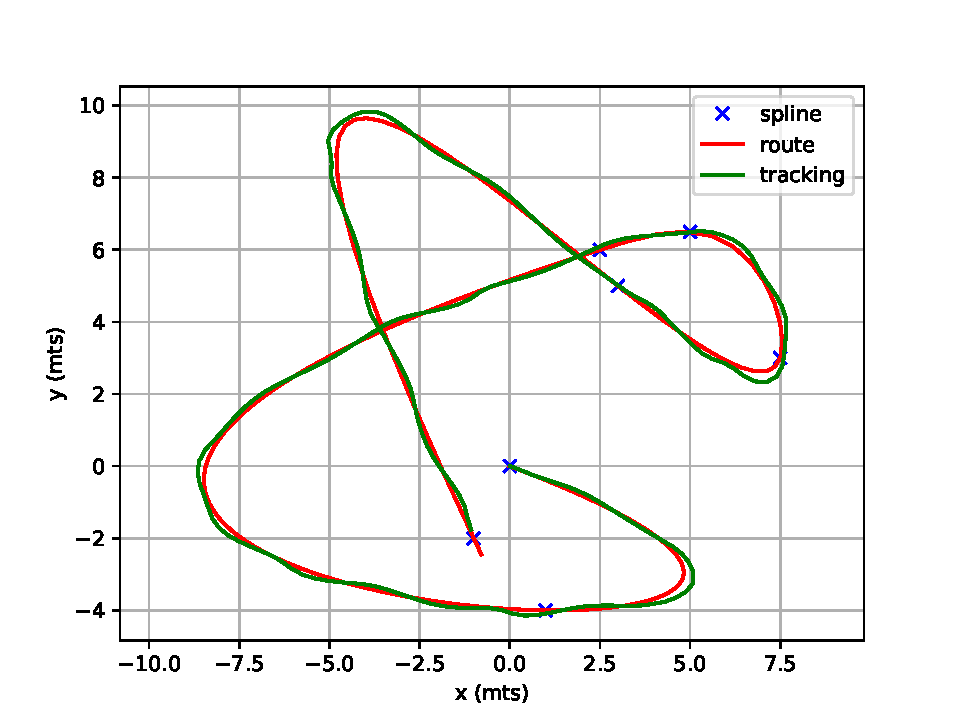
\includegraphics[width=60mm]{img/3r5fmA.pdf}}
     \caption{Plot for the best simulations on Track A.}
        \label{fig:3RutasA}
\end{figure}
\begin{paracol}{2}
\linenumbers
\switchcolumn


%The optimization of fuzzy controllers for real-world applications requires a
%broader perspective, optimization needs to consider more variables 
% paragraph (?4:_:\lam) (end)% Broader than what? - JJ
  % If this is future work, move it there - JJ

%Our literature review
%shows that using only the RMSE is a common practice but could not be enough for
%this type of application. % Probably redundant. In this section you need to
                          % discuss why using other metrics helped find a better
                          % solution - jj

% This should be a bit more precise and address the possible
% shortcomings. Making things in parallel need not make it faster - JJ

Furthermore, because of the high computational cost, as future work, we will
propose a technique to execute these experiments in a distributed way, adding
multiple populations such as the island-model, or a pool-based evolutionary
approach, that could enhance the search, giving supralinear execution times.
Later we could try other bio-inspired methods and compare the results. We could
also add more membership functions and test other functions to improve the
inference system.


%%%%%%%%%%%%%%%%%%%%%%%%%%%%%%%%%%%%%%%%%%%\section{Conclusions}

%This section is not mandatory, but can be added to the manuscript if the
%discussion is unusually long or complex.

%%%%%%%%%%%%%%%%%%%%%%%%%%%%%%%%%%%%%%%%%%
%\section{Patents}
%
%This section is not mandatory, but may be added if there are patents resulting
%from the work reported in this manuscript.
%
%%%%%%%%%%%%%%%%%%%%%%%%%%%%%%%%%%%%%%%%%%
\vspace{6pt} 

%%%%%%%%%%%%%%%%%%%%%%%%%%%%%%%%%%%%%%%%%%
%% optional
%\supplementary{The following are available online at \linksupplementary{s1}, Figure S1: title, Table S1: title, Video S1: title.}

% Only for the journal Methods and Protocols:
% If you wish to submit a video article, please do so with any other supplementary material.
% \supplementary{The following are available at \linksupplementary{s1}, Figure S1: title, Table S1: title, Video S1: title. A supporting video article is available at doi: link.} 

%%%%%%%%%%%%%%%%%%%%%%%%%%%%%%%%%%%%%%%%%%

\authorcontributions{
Conceptualization, A.M., M.G, and O.C.;
methodology, A.M.; software, M.G.; validation, O.C. and J.M.; data curation, A.M.;
writing---original draft preparation, A.M.; writing---review and editing, M.G. and J.M ;
visualization, A.M.; supervision, O.C.; All authors have read and agreed to the published version of
the manuscript.}

\funding{This research was funded by projects TecNM-5654.19-P and DemocratAI PID2020-115570GB-C22.}

\institutionalreview{Not applicable}

\informedconsent{Not applicable} 

\dataavailability{All data and code is available with an open source license from \url{https://github.com/mariosky/fuzzy-control}} 

%\acknowledgments{In this section you can acknowledge any support given which is not covered by the author contribution or funding sections. This may include administrative and technical support, or donations in kind (e.g., materials used for experiments).}

\conflictsofinterest{``The authors declare no conflict of interest.''} 


%%%%%%%%%%%%%%%%%%%%%%%%%%%%%%%%%%%%%%%%%%
%% Only for journal Encyclopedia
%\entrylink{The Link to this entry published on the encyclopedia platform.}

%%%%%%%%%%%%%%%%%%%%%%%%%%%%%%%%%%%%%%%%%%
%% Optional
%\abbreviations{Abbreviations}{
%The following abbreviations are used in this manuscript:\\
%
%\noindent 
%\begin{tabular}{@{}ll}
%MDPI & Multidisciplinary Digital Publishing Institute\\
%DOAJ & Directory of open access journals\\
%TLA & Three letter acronym\\
%LD & Linear dichroism
%\end{tabular}}
%
%%%%%%%%%%%%%%%%%%%%%%%%%%%%%%%%%%%%%%%%%%
\end{paracol}
%%%%%%%%%%%%%%%%%%%%%%%%%%%%%%%%%%%%%%%%%%
% To add notes in main text, please use \endnote{} and un-comment the codes below.
%\begin{adjustwidth}{-5.0cm}{0cm}
%\printendnotes[custom]
%\end{adjustwidth}
%%%%%%%%%%%%%%%%%%%%%%%%%%%%%%%%%%%%%%%%%%
\reftitle{References}

% Please provide either the correct journal abbreviation (e.g. according to the “List of Title Word Abbreviations” http://www.issn.org/services/online-services/access-to-the-ltwa/) or the full name of the journal.
% Citations and References in Supplementary files are permitted provided that they also appear in the reference list here. 

%=====================================
% References, variant A: external bibliography
%=====================================
\externalbibliography{yes}
\bibliography{tracking}

\end{document}


